% mnras_template.tex 
%
% LaTeX template for creating an MNRAS paper
%
% v3.0 released 14 May 2015
% (version numbers match those of mnras.cls)
%
% Copyright (C) Royal Astronomical Society 2015
% Authors:
% Keith T. Smith (Royal Astronomical Society)

% Change log
%
% v3.0 May 2015
%    Renamed to match the new package name
%    Version number matches mnras.cls
%    A few minor tweaks to wording
% v1.0 September 2013
%    Beta testing only - never publicly released
%    First version: a simple (ish) template for creating an MNRAS paper

%%%%%%%%%%%%%%%%%%%%%%%%%%%%%%%%%%%%%%%%%%%%%%%%%%
% Basic setup. Most papers should leave these options alone.
\documentclass[fleqn,usenatbib]{mnras}

% MNRAS is set in Times font. If you don't have this installed (most LaTeX
% installations will be fine) or prefer the old Computer Modern fonts, comment
% out the following line
\usepackage{newtxtext,newtxmath}
% Depending on your LaTeX fonts installation, you might get better results with one of these:
%\usepackage{mathptmx}
%\usepackage{txfonts}

% Use vector fonts, so it zooms properly in on-screen viewing software
% Don't change these lines unless you know what you are doing
\usepackage[T1]{fontenc}
\usepackage{float}
\usepackage{enumerate}

% Allow "Thomas van Noord" and "Simon de Laguarde" and alike to be sorted by "N" and "L" etc. in the bibliography.
% Write the name in the bibliography as "\VAN{Noord}{Van}{van} Noord, Thomas"
\DeclareRobustCommand{\VAN}[3]{#2}
\let\VANthebibliography\thebibliography
\def\thebibliography{\DeclareRobustCommand{\VAN}[3]{##3}\VANthebibliography}


%%%%% AUTHORS - PLACE YOUR OWN PACKAGES HERE %%%%%

% Only include extra packages if you really need them. Common packages are:
\usepackage{graphicx}	% Including figure files
\usepackage{amsmath}	% Advanced maths commands
% \usepackage{amssymb}	% Extra maths symbols
\usepackage{subfigure}
\usepackage{siunitx}
\usepackage{array}
%%%%%%%%%%%%%%%%%%%%%%%%%%%%%%%%%%%%%%%%%%%%%%%%%%

%%%%% AUTHORS - PLACE YOUR OWN COMMANDS HERE %%%%%

% Please keep new commands to a minimum, and use \newcommand not \def to avoid
% overwriting existing commands. Example:
%\newcommand{\pcm}{\,cm$^{-2}$}	% per cm-squared

%%%%%%%%%%%%%%%%%%%%%%%%%%%%%%%%%%%%%%%%%%%%%%%%%%

%%%%%%%%%%%%%%%%%%% TITLE PAGE %%%%%%%%%%%%%%%%%%%

% Title of the paper, and the short title which is used in the headers.
% Keep the title short and informative.
\title[Evolution of mass density profile]{'$10\text{kpc}$ collar' -- probing the evolution of early-type galaxies by focusing its inner mass density profile}

% The list of authors, and the short list which is used in the headers.
% If you need two or more lines of authors, add an extra line using \newauthor
\author[Rongfu Liu et al.]{
Rongfu Liu$^{1}$, 
Alessandro Sonnenfeld$^{1}$\\
$^{1}$Department of Astronomy, School of Physics and Astronomy, Shanghai Jiao Tong University, Shanghai, China
% List of institutions
}

% These dates will be filled out by the publisher
\date{Accepted XXX. Received YYY; in original form ZZZ}

% Enter the current year, for the copyright statements etc.
\pubyear{2023}

% Don't change these lines
\begin{document}
\label{firstpage}
\pagerange{\pageref{firstpage}--\pageref{lastpage}}
\maketitle

% Abstract of the paper
\begin{abstract}
Early-type galaxies (ETGs) today is believed to have experienced more dramatic growth in their evolution history, comparing with their star-forming counterpart. The underlying mechanism of the evolution of ETGs,which is still not been well-understood yet, could be inferred by tracing its impact on various properties of galaxies, among which the mass density profile is one that has not drawn much attention in literature. 
% Traditionally, most of the method used to investigate the evolution of these object involved the total light of one galaxy, which we believed to be not well-defined and is likely to suffer from extrapolation problem. To eliminate such potential bias
In this work, we aim to investigate the evolution of ETGs by focusing on the mass density profile inside a fixed aperture, $10$kpc. 
We use a new parameterization, namely $M_{*,10}$ and $\Gamma_{*,10}$ which is the mass and the mass-weighted density slope enclosed in circularised aperture $10$kpc respectively, to capture the feature of mass density profile in such inner region and then probe its evolution trend. We first explore the $\Gamma_{*,10} - M_{*,10}$ relation for a sample of quiescent galaxies from GAMA survey combining with the KiDs image, and find a steeper slope of the $\Gamma_{*,10} - M_{*,10}$ relation for galaxies with lower redshift. We then analyzed a collection of binary-merger simulations which contains mergers with different merger mass ratio. From the simualtion result we could directly observe that mergers would always induce a decrease in $\Gamma_{*,10}$ , but might induce a counter-intuitive increase in $M_{*,10}$ for larger galaxies and smaller merger mass ratio. We then built a toy model to predict the evolution in $\Gamma_*{*,10} - M_{*,10}$ relation, and found that for every merger mass ratio, the slope would always increase and the normalization would always decrease, while the change would become more intensive for smaller merger mass ratio. Comparing with the observation result, we believe galaxies do grow during redshift range $0.15 \leq z \leq 0.40$, and the growth should be driven by mergers with merger mass ratio lower than 1:5.
% analyses a collection of binary-merger simulations and find that the growth in $M_{*,10}$ and $\Gamma_{*,10}$ are different in different merger scenarios and different galaxies size. We then select a $M_{*,10}$ complete sample of galaxies in GAMA survey and use KiDs r-band image to provide structural parameters. We measured $M_{*,10}$ and $\Gamma_{*,10}$ for these galaxies, and compare the evolutionary trend with simulation results. We find that for galaxies with $M_{*,10} \geq 10^{10.9} M_{\odot}$ and redshift $0.15 \leq z \leq 0.40$, no significant evidence shows they experienced a growth due to merger of any kinds.  
\end{abstract}

% Select between one and six entries from the list of approved keywords.
% Don't make up new ones.
\begin{keywords}
    galaxies: elliptical and lenticular, cD -- galaxies: evolution -- galaxies: structure
\end{keywords}

%%%%%%%%%%%%%%%%%%%%%%%%%%%%%%%%%%%%%%%%%%%%%%%%%%

%%%%%%%%%%%%%%%%% BODY OF PAPER %%%%%%%%%%%%%%%%%%

\section{Introduction}
Early type galaxies (ETGs), which are, by definition, typically elliptical in shape, are believed to be the end product of galaxy formation and evolution process and have completed most of their star-forming activities by the time that being observed. The passive evolution process of ETGs is a key problem in astrophysics. Obtaining a better understanding on this process could help us better understand the hierarchical structure formation theory, which is fundamental in $\Lambda$CDM cosmology.
\par Over the past few decades, observations have suggested that ETGs at higher redshift (i.e. $z\approx 2$) have significant differences from their $z \approx 0 $ counterpart in many aspects. For instance, ETGs at higher redshift are more compact in size \citep[e.g.][]{daddiPassivelyEvolvingEarlyType2005, toft2007, trujillo2006, trujillo2007, vandokkum2008} and more homogeneous in color gradient, i.e. the contrast in color between the outskirt and the center is less significant than their low-redshift counterparts
% the outskirt of ETGs becomes bluer in comparison with its center
 \citep[e.g.][]{Suess2019a,Suess2019b,Suess2020}. 
%  In particular, the evolution process of such quiescent, ultra compact objects experienced are believed to have induced a dramatic growth in size by a factor of about 3 between $z = 2$ and $z = 0$ \citep[e.g.][]{fan_dramatic_2008,  van_dokkum_growth_2010,vanderwel3DHSTCANDELSEvolution2014,damjanov2019,  hamadouche2022}. 
In particular, the size growth of such quiescent, ultra compact objects induced by the passive evolution process is believed to be a factor of about 3 between $z = 2$ and $z = 0$ \citep[e.g.][]{fan_dramatic_2008,  van_dokkum_growth_2010,vanderwel3DHSTCANDELSEvolution2014,damjanov2019,hamadouche2022}.
 Combining with the fact that the star formation rate of ETGs are relatively low, it is suggested that the these galaxies should have experienced a built-up process of their outer envelope since $z \approx 1.5$ via some form of merging and accretion~\citep[e.g.][]{hopkins2009,hopkins2010,van_dokkum_growth_2010} . Numerous works in literature that based on both observations and hydrodynamic simulations have suggested that among various possible mechanisms, the major one should be the dissipationless dry mergers, especially for mergers with a relatively small mass ratio between the accreted galaxy and the progenitor galaxy (hereafter minor merger).The rationale is that the minor merger is more promising in qualitatively reproducing the evolution trend in size, central densities and orbital structures of these quiescent galaxies.
\citep[e.g.][]{naab_minor_2009, van_dokkum_2010_hubble, oser_cosmological_2011, newman2012, hilz_how_2013, dekel_wet_2014, deugenio2023}. Recently, taking the advantage of the depth and resolution of JWST Advanced Deep Extragalatic Survey \citep{Gardner_JWST,Eisenstein_JADES}, it is suggested that minor merger also have the potential to contribute the color gradient evolution of ETGs \citep{Suess2023}.
\par However, if we investigate the evolution process quantitatively, we would find one of the problems in this field is that the minor merger scenario is not sufficient to explain the entire growth of ETGs at redshift $z > 1$. Works in literature that based on HST images could be an example.They identified satellite galaxies around massive ETGs and found that the merging event of ETGs with their surrounding satellites could only account for at most a half of the entire size growth \citep{newman2012,Belli_2015}. Moreover, works based on theoretical model also implies that if we aiming at explaining the size growth of ETGs by solely invoking minor mergers, the scatter in the scaling relation ($M_*-R_e$ relation) of ETGs would become larger and thus inconsistent with observation~\citep{nipoti2009,nipoti12}. Fortunately, some possible solutions to this problem have already been proposed. Given the fact that the observed size of star-forming galaxies are on average larger than quiescent ones ~\citep[e.g.][]{newman2012,vanderwel3DHSTCANDELSEvolution2014,Belli_2015,KiDs_Roy}, the joining of newly quenched ex-star-forming galaxies to the population of ETGs could be a possible supplement to the size growth of ETGs ~\citep[e.g.][]{van_dokkum_1996,vandokkumMorphologicalEvolutionAges2001,carolloNEWLYQUENCHEDGALAXIES2013,fagioliMinorMergersProgenitor2016}. In addition, the existence of color gradient could also mimic the observed size growth of ETGs, thus mislead to a conclusion that the minor merger scenario is insufficient~\citep{Suess2019a,Suess2019b}.
% Or on the other hand, the size growth might have been overestimated due to the ignorance on the color gradient of ETGs, which would also result in the insufficiency of minor merger ~\citep{Suess2019a,Suess2019b}.
 Nevertheless, detailed theoretical models that could take various possible scenarios into account and explain the entire growth of ETGs is still missing.


% Earlier work based on HST images detected satellite galaxies around massive ETGs with mass ratio larger than $1:10$, and suggested part of the size growth of these ETGs could be a consequence of the merging with their surrounding satellites \citep{newman2012, Belli_2015}. Recently, taking the advantage of the depth and resolution of JWST Advanced Deep Extragalatic Survey \citep{Gardner_JWST,Eisenstein_JADES}, it is now possible to detect very low mass ratio ($ \leq 1:100$) mergers. The result is in broad agreement in the mass ratio range that is overlapped with literature
% with the previous work in higher merger mass ratio range 
% ($ > 1:10$), while extend our knowledge to the lower mass ratio range and suggests that the color gradients evolution could also be explained by minor mergers event in this range\citep{Suess2023}.
% \par However, the evolution of ETGs is still not well understood. One of the remaining problem is that the growth mechanisms are still under debate. Although minor merger is believed to be a much promising mechanism,
% % as it is in general consistent with evolution trend of ETGs in some aspect, there are still some issues remain unsolved. For instance, as is mentioned above, minor merger are 
% it seems to be insufficient to reproduce the entire size growth of ETGs, especially at higher redshift $z > 1$. If we aiming at explaining the size growth of ETGs by solely invoking minor mergers, the amount of mass growth due to mergers would not be consistent with neither theoretical prediction \citep{nipoti12} nor the observation result \citep{newman2012}. Given the fact that the observed size of star-forming galaxies are on average larger than quiescent ones \citep[e.g.][]{newman2012,vanderwel3DHSTCANDELSEvolution2014,Belli_2015,KiDs_Roy}, the joining of newly quenched ex-star-forming galaxies to the population of ETGs could be a possible supplement to the size growth of ETGs \citep[e.g.][]{van_dokkum_1996,vandokkumMorphologicalEvolutionAges2001,carolloNEWLYQUENCHEDGALAXIES2013,fagioliMinorMergersProgenitor2016}. Or on the other hand, the size growth might have been overestimated due to the ignorance on the color gradient of ETGs, which would also result in the insufficiency of minor merger \citep{Suess2019a,Suess2019b}. Nevertheless, detailed theoretical models that could take various possible scenarios into account and explain the entire growth of ETGs is still in absence. 
\par Another problem occurs at relatively lower redshift $z \leq 1$, the observed evolution of ETGs at that epoch do not converge in some degree. The growth rate of ETGs at that time  seems to be mass-dependent. \cite{vanderwel3DHSTCANDELSEvolution2014,KiDs_Roy} suggested a more rapid size growth rate for more massive ETGs ($M_* \geq 10^{11} M_\odot$), while is not in consistent with \cite{damjanov2019}, which found that less massive ETGs tends to grow faster. Moreover, effort on exploring the number density growth of ETGs implies a lack of growth in the stellar mass function in the same redshift interval \citep[e.g.][]{Bundy2017,Kawinwanichakij2020}, which is in general in agreement with~\cite{damjanov2019} as they both imply that massive ETGs do not grow significantly, and thus in contrast with~\cite{vanderwel3DHSTCANDELSEvolution2014} and~\cite{KiDs_Roy}. Such complexity limit our ability to make precise conclusion on the evolution of ETGs in this redshift range. Whether the ETGs grow in this redshift range is still not determined, let alone the detailed growth mechanism. 
\par Besides the traditional size and mass, which is often represented by effective radius $R_e$ and $M_*$, another quantity that might could also reflect the evolution of ETGs is the mass distribution, or in another word, the density profile, as the evolution process would indeed leave impact on it. For instance, \cite{sonnenfeld2014} has measured this quantity using lensing data, and this work is proved to be a success in providing a new evidence on the insufficiency of minor merger scenario. In fact, switching to a new perspective is sometimes essential, as some new information may be difficult to be obtained by traditional methods. To provide an additional perspective, we choose to focus on the inner region of ETGs, in supplement to some previous effort on measuring the outer properties of galaxies and their evolution \citep[e.g.][]{Huang2020}. 

%  One possible perspective in investigating the evolution of ETGs could be separating galaxies into outer region and inner region, and focusing one of them. Previously,~\cite{Huang2020} has done some effort on measuring the outer properties of galaxies and their evolution.

% \par Besides the growth in size and mass that is often summarized by effective radius $R_e$ and total stellar mass $M_*$, one parameter the might have not drawn much focus in literature is the mass (or light) distribution, or in another word, the density profile. This quantity is also able to place constrains on the evolution of ETGs, as it has indeed been altered during the evolution process. For instance, utilizing the lensing observations, \cite{sonnenfeld2014} measured the mass density profile slope of ETGs and provide an additional evidence on the insufficiency of minor merger scenario. In fact, the knowledge about the evolution in density profile have a large potential to improve our understanding in ETGs evolution, as switching to a new perspective may provide us some valuable additional information that are unable to obtain previously. 
\par Following \cite{Alessandro20}, we define the 'inner region' as the region that inside a circularized radius, $10kpc$, and focus on the mass profile using the mass ($M_{*,10}$) and mass-weighted density slope ($\Gamma_{*,10}$) that enclosed in the inner region. The later is defined as  
% we choose to focus the inner mass profile using the mass enclosed within $10 \text{kpc}$, $M_{*,10}$, as well as mass-weighted density slope enclosed in the same aperture, $\Gamma_{*,10}$, to address this issue.The second parameter is defined as
\begin{equation}
    \label{eq:gammastar10}
    \Gamma_{*,10} = \frac{2\pi \int_0^{10} R \frac{dlog\Sigma_*}{dlogR}\Sigma_*(R)dR}{2\pi \int_0^{10}R\Sigma_*(R)dR} = 2 - \frac{2\pi \times 10^2 \times \Sigma_*(10)}{M_{*,10}}
\end{equation} 
Setting a certain value to these two parameters, the mass profile inside $10 \text{kpc}$ could be described precisely \citep[see Fig.8 in][]{Alessandro20}, we hence believe this parameterization is reliable to be used in probing the evolution of inner mass profile. In fact, a benefit of using this parameterization is that it could avoid the potential bias introduced by "extrapolation problem", which might arise when one try to obtain some quantities, such a the total light of one galaxy, by extrapolating the surface brightness model to outer region as the model itself is not well constrained by reliable data there.
% fit a surface brightness model to observed galaxies and extrapolate the model to outer region that is not well constrained by the data.
 Traditional parameters, such as $R_e$ and $M_*$, however, are both sensitive to this problem, thus we believe that they are not as robust as $M_{*,10}$ and $\Gamma_{*,10}$. With the help of our new robust parameterization, our main goal in this paper is to probe the evolution of the inner density profile of ETGs in the redshift range $0.15 \leq z \leq 0.40$. Given the literature uncertainty in that redshift range, we would first try to answer whether the inner mass profile of ETGs would evolve, and then try to infer the growth mechanism in details.
\par To achieve this goal, it's necessary to understand the impact of various growth mechanism, in particular, mergers with diferent merger ratio.
%  we can obtain a strict relation between $\Delta M_*$ and $\Delta R_e$ depending on different merger scenarios
%  It is non-trivial to derive the relation in $\Delta M_{*,10}$ and $\Delta \Gamma_{*,10}$ analytically as a fixed aperture size 10kpc is involved while the size of galaxies may vary. Nevertheless, N-body simulations can be helpful. 
 We thus utilize the simulation result from \cite{nipoti2009} which contains a number of binary mergers with different mass ratio. We measure the $M_{*,10}$ and $\Gamma_{*,10}$ of both progenitor and merger remnant and calculate the growth in these two quantities. In addition to finding that different merger ratio behaves differently, we discovered that the scale of galaxy also make diferences. With the knowledge on how mergers will evolve galaxies in $M_{*,10}, \Gamma_{*,10}$ space, we thus proposed a simple toy model on how different merger scenarios would affect the relation between $\Gamma_{*,10}$ and $M_{*,10}$. We then turn to the observation data in order to make comparison between with our toy model and thus build a intuitive understanding on what could be the possible growth mechanism of ETGs. 
 . We select ETGs from GAMA DR4 main survey (Galaxy and Mass Assembly, \cite{GAMAmain};\cite{bellstedt_galaxy_2020} ; \cite{GAMA1}; \cite{GAMA2}) and obtained precise spectroscopic redshift and other quantities that related to spectrum measurement, e.g. stellar mass. In addition, 
% we use the 2DPHOT structural parameter catalogue from KiDs DR4 We then compared them with the evolution of these two quantities in reality
the structural parameter are measured from KiDs photometry (Kile Degree survey , \cite{kuijken_fourth_2019}, \cite{KiDs_Roy}, \cite{Amaro_rejection_2021}) using GalNet (\cite{GaLNet2022}). Based on these observation datas,  we then calculated their $M_{*,10} $ and $\Gamma_{*,10}$ and further analyse the , $M_{*,10} - \Gamma_{*,10}$ relation and their evolution from $z = 0.4$ to $z = 0.15$. We then compared the observation result with the predicted one from our toy model and thus infer the growth mechanism of ETGs in this redshift range.
\par The structure of this paper is as follows. We present the selection of our observational sample and the observed $\Gamma_{*,10} - M_{*,10}$ relation in Sect.\ref{sec:2}. In Sect.\ref{sec:3}, we present the details of the simulation and the toy model that we built upon the simulation, as well as the comparison between observations. Then we discussed the result in Sect.\ref{sec:4} and give a brief conclusion in Sect.\ref{sec:5}.
\par In this paper, we assume a flat $\Lambda$CDM cosmology with $\Omega_M = 0.3$ and $H_0 = 70 km ~s^{-1}~Mpc^{-1}$. Magnitude are in AB units and stellar mass are in solar units.
% suggests that mergers with ratio close to 1:10 are likely to drive the size growth while lower mass ratio mergers might dominate the color gradients evolution \citep{Suess2023}.
% In particular, minor mergers, which means the mass ratio between the accreted galaxy and the progenitor galaxy is relatively small, are believed to have dominated the merger event that one galaxy might experience 
% \par Obtained the knowledge on how mergers will evolve galaxies in $M_{*,10}, \Gamma_{*,10}$ space, we turn to observation data to investigate how do these two parameter grow in real world and attempting to infer the growth mechanism from the observational result. We select galaxies from GAMA survey and use KiDs r-band image to provide a S\'{e}rsic surface brightness fitting. We use a spectroscopic index $D_n 4000$ to distinguish quiescent galaxies from star-forming ones. In order to avoid bias introduced by the incompleteness of the sample, we define a redshift-dependent completeness cut on $M_{*,10}$ and exclude those galaxies whose $M_{*,10}$ is lower than this completeness limit, thus obtain the sample that are at least $95\%$ complete in $M_{*,10}$. In addition, we further exclude some low redshift galaxies in consideration of cosmic variance. The final sample we utilized to investigate the evolution trend is shown in Fig.\ref{fig:completeness_cut} as cyan dots.
% \par Using the S\'{e}rsic parameter provided by KiDs, in particular, using a CNN methods namely GalNet (\cite{GaLNet2022}), we measured the $M_{*,10}$ and $\Gamma_{*,10}$ following the procedure that has been described in Sect.\ref{sec:cal}. In addition, we operate a small modification to ensure the consistency between the stellar mass and S\'{e}rsic parameter. We then divide the sample into four redshift bins and five $M_{*,10}$ bins, and calculate the median value of $\Gamma_{*,10}$ in each bin. The result is shown in Fig.\ref{fig:mg_relation} and Fig.\ref{fig:gamma}.We can tell from these two figures that neither the $M_{*,10} - \Gamma_{*,10}$ relation nor the $\Gamma_{*,10} - z$ relation shows a significant evolution trend. Having compared with the knowledge that we have obtained from simulations result, we conclude that galaxies with $M_{*,10}$ larger than  $10^{10.9} M_{\odot}$ do not experience significant growth due to mergers in the redshift range $0.15 \leq z \leq 0.4$.
% \par In conclusion, our work provide a robust way to make direct comparison between observation data and simulation result. Moreover, as the different behaviour of $M_{*,10}$ and $\Gamma_{*,10}$ during different mergers processes, our method also provide a new way to distinguish the growth mechanism of quiescent galaxies. At meanwhile, this method might have its limitation in studying less massive quiescent galaxies as our requirement of accurate physical aperture $10$kpc need the spectrum of galaxies to be measured, while the facilities of spectroscopic surveys limit our ability to detect fainter and more distant galaxies. As a consequence, although we have used the most advanced observational project GAMA and KiDs, we can only apply our method to galaxies with $M_{*,10} $ no less than $10^{10.9} M_{\odot}$ and redshift $z$ lies between a relatively narrow range $0.15 \leq z \leq 0.4$. Fortunately, numbers of stage-IV surveys are under construction, e.g. CSST(China Space Station telescope, \cite{csst}), Euclid (\cite{Euclid}) and JWST(ADD CITE HERE). These surveys have stronger ability to detect fainter objects, thus could enrich the sample of quiescent galaxies and broaden the range of $<_{*,10}$ and $z$. Hopefully, applying our method to these new data could provide us more detailed information on the growth of quiescent galaxies in a more robust way. 

% Figures and tables should be placed at logical positions in the text. Don't
% worry about the exact layout, which will be handled by the publishers.

% Figures are referred to as e.g. Fig.~\ref{fig:example_figure}, and tables as
% e.g. Table~\ref{tab:example_table}.

% % Example figure
% \begin{figure}
% 	% To include a figure from a file named example.*
% 	% Allowable file formats are eps or ps if compiling using latex
% 	% or pdf, png, jpg if compiling using pdflatex
% 	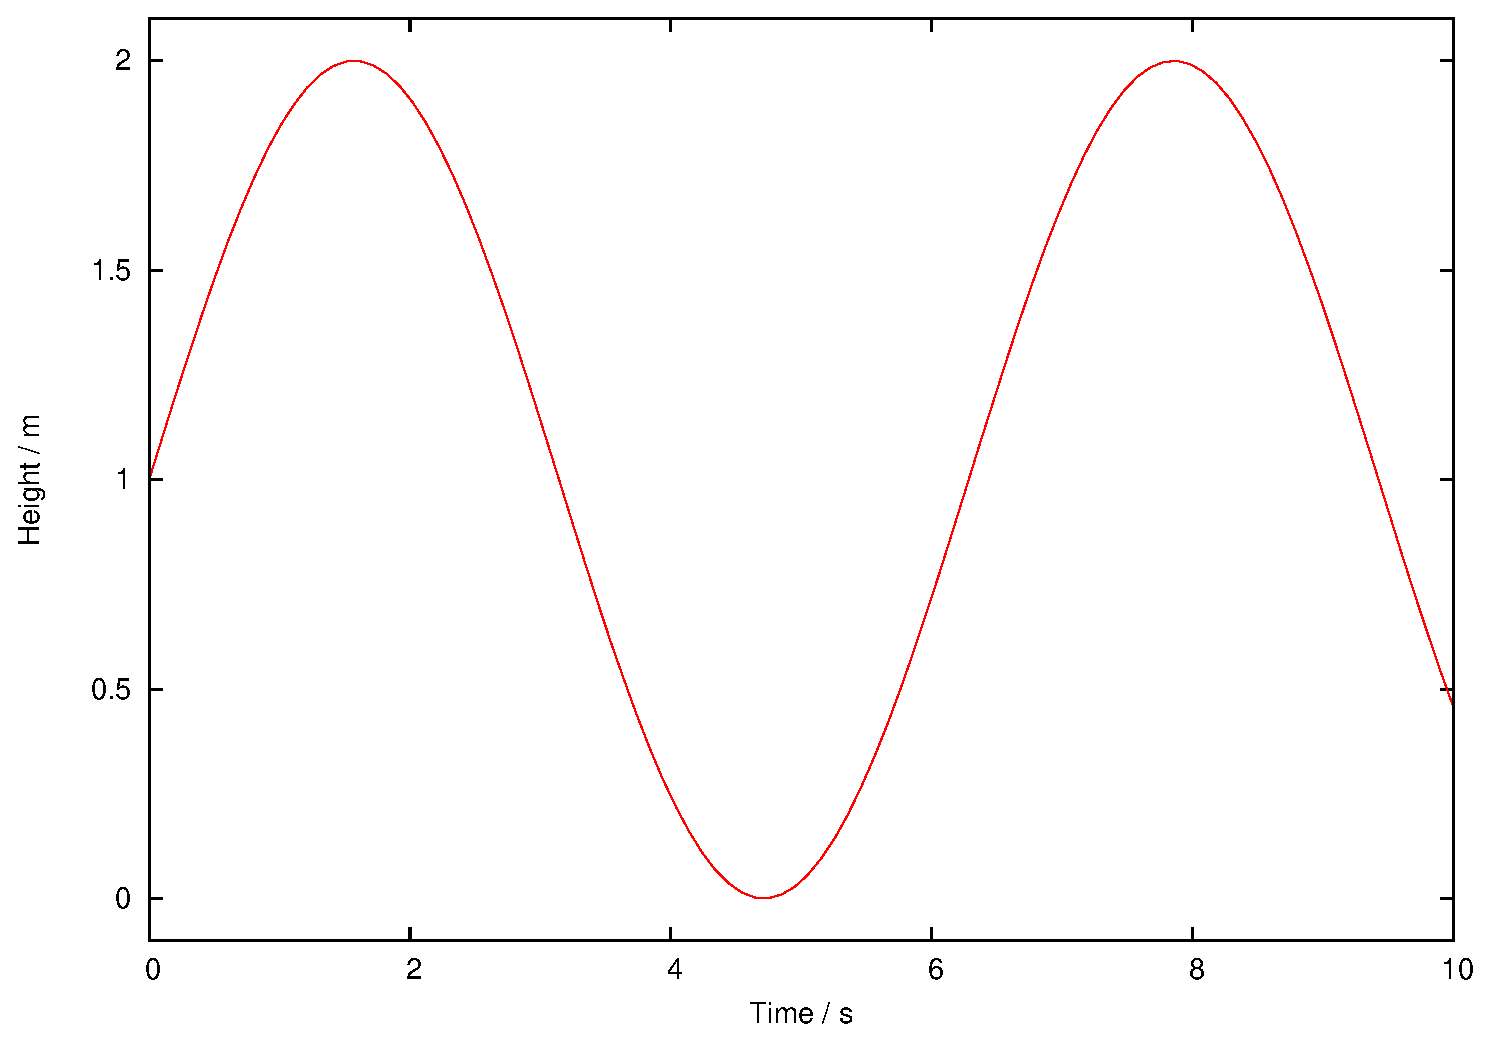
\includegraphics[width=\columnwidth]{example}
%     \caption{This is an example figure. Captions appear below each figure.
% 	Give enough detail for the reader to understand what they're looking at,
% 	but leave detailed discussion to the main body of the text.}
%     \label{fig:example_figure}
% \end{figure}

% % Example table
% \begin{table}
% 	\centering
% 	\caption{This is an example table. Captions appear above each table.
% 	Remember to define the quantities, symbols and units used.}
% 	\label{tab:example_table}
% 	\begin{tabular}{lccr} % four columns, alignment for each
% 		\hline
% 		A & B & C & D\\
% 		\hline
% 		1 & 2 & 3 & 4\\
% 		2 & 4 & 6 & 8\\
% 		3 & 5 & 7 & 9\\
% 		\hline
% 	\end{tabular}
% \end{table}


% \section{Conclusions}

% The last numbered section should briefly summarise what has been done, and describe
% the final conclusions which the authors draw from their work.

% \section*{Acknowledgements}

% The Acknowledgements section is not numbered. Here you can thank helpful
% colleagues, acknowledge funding agencies, telescopes and facilities used etc.
% Try to keep it short.

% %%%%%%%%%%%%%%%%%%%%%%%%%%%%%%%%%%%%%%%%%%%%%%%%%%
% \section*{Data Availability}

 
% The inclusion of a Data Availability Statement is a requirement for articles published in MNRAS. Data Availability Statements provide a standardised format for readers to understand the availability of data underlying the research results described in the article. The statement may refer to original data generated in the course of the study or to third-party data analysed in the article. The statement should describe and provide means of access, where possible, by linking to the data or providing the required accession numbers for the relevant databases or DOIs.




% %%%%%%%%%%%%%%%%%%%% REFERENCES %%%%%%%%%%%%%%%%%%

% % The best way to enter references is to use BibTeX:
\newpage
\bibliographystyle{mnras}
\bibliography{example} % if your bibtex file is called example.bib

% % Alternatively you could enter them by hand, like this:
% % This method is tedious and prone to error if you have lots of references
% %\begin{thebibliography}{99}
% %\bibitem[\protect\citeauthoryear{Author}{2012}]{Author2012}
% %Author A.~N., 2013, Journal of Improbable Astronomy, 1, 1
% %\bibitem[\protect\citeauthoryear{Others}{2013}]{Others2013}
% %Others S., 2012, Journal of Interesting Stuff, 17, 198
% %\end{thebibliography}

% %%%%%%%%%%%%%%%%%%%%%%%%%%%%%%%%%%%%%%%%%%%%%%%%%%

% %%%%%%%%%%%%%%%%% APPENDICES %%%%%%%%%%%%%%%%%%%%%

% \appendix

% \section{Some extra material}

% If you want to present additional material which would interrupt the flow of the main paper,
% it can be placed in an Appendix which appears after the list of references.

%%%%%%%%%%%%%%%%%%%%%%%%%%%%%%%%%%%%%%%%%%%%%%%%%%


% Don't change these lines
\bsp	% typesetting comment
\label{lastpage}
\end{document}

% End of mnras_template.tex
